\chapter{Convolutional Neural Networks}\label{ch:cnn}
Convolutional Neural Networks (CNNs) are a group of models which allow for efficient training on high dimensional data.
This is especially useful in the field of computer vision as image data is fundamentally high dimensional.

\begin{figure}[H]
    \centering
    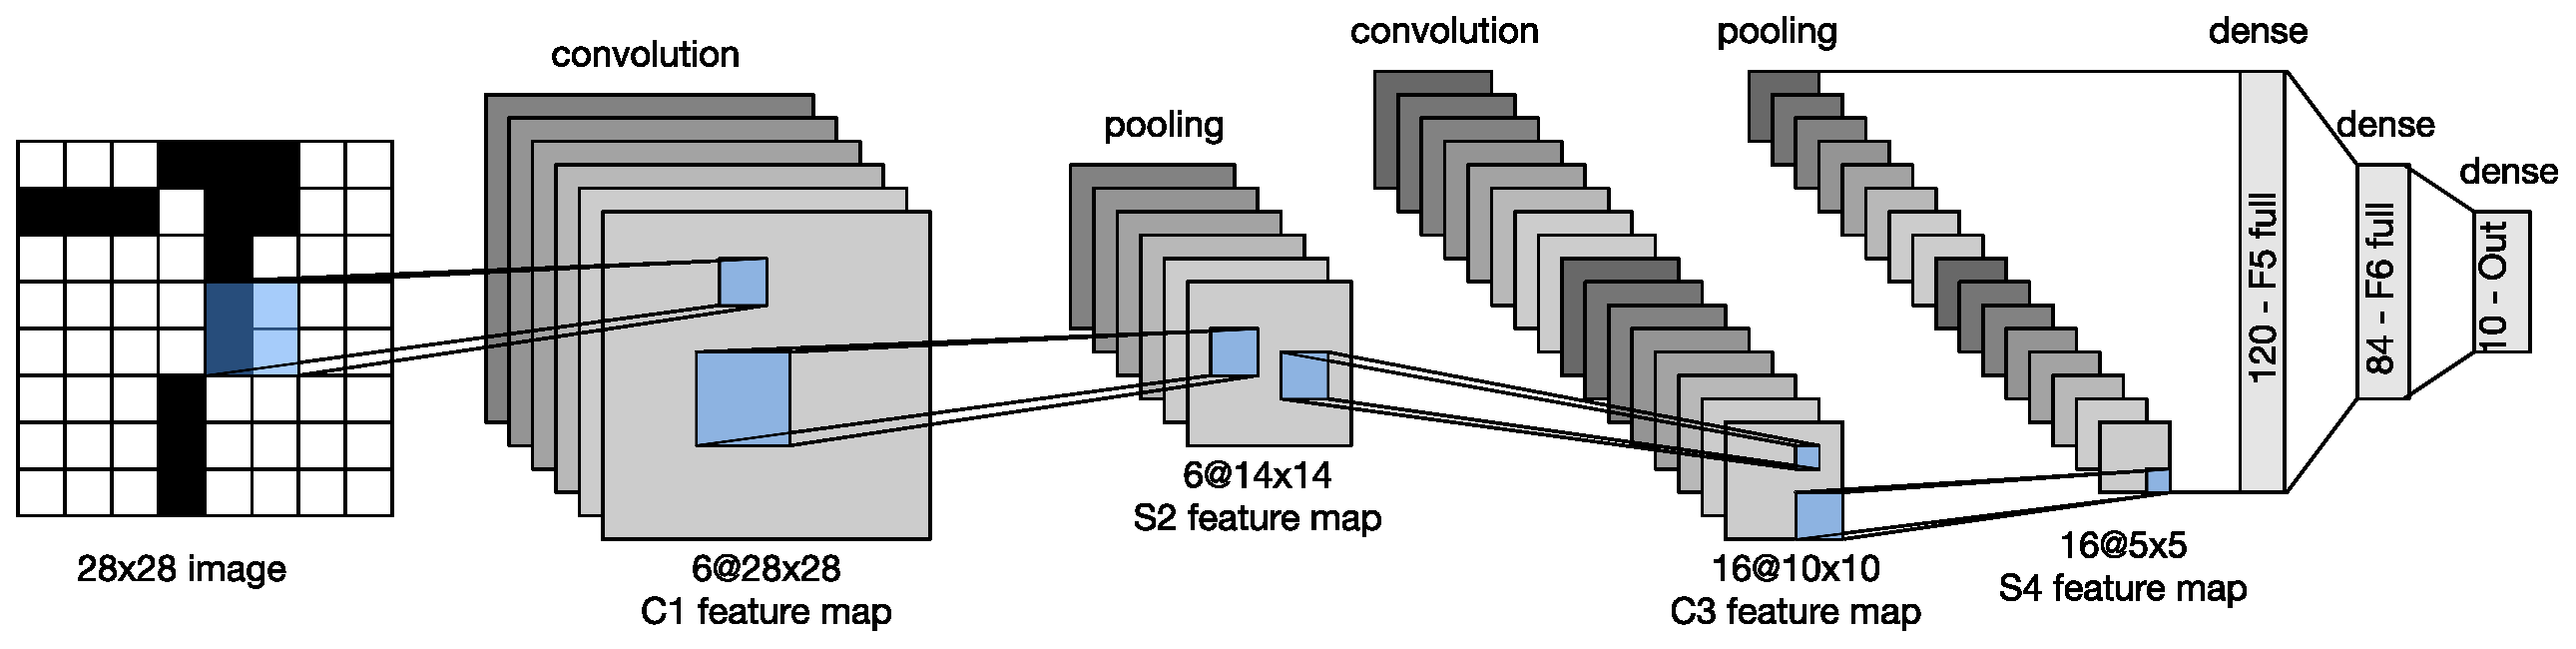
\includegraphics[width=\columnwidth]{images/cnn/lenet.eps}
    \caption{Example of CNN model (LeNet 5)~\cite{CNN}}
    \label{fig:cnn}
\end{figure}

The image~\ref{fig:cnn} is an illustration of one of the oldest CNN models \textit{LenNet 5} which was used for
handwritten character recognition.
As we can see, there are many layers stacked in the model's architecture.
This is typical for CNNs and it's a reason why CNNs belong to the class of machine learning methods called
\textit{deep learning}\footnote{Set of machine learning models with
\textit{credit assignment path (CAP)} higher than 2.
The CAP is the chain of transformations from input to output.}
Usually there are three layer types in the CNN model: \textit{dense}~\ref{sec:dense},
\textit{convolutional}~\ref{sec:convolutional} and \textit{pooling}~\ref{sec:pooling}.

\section{Dense layer}\label{sec:dense}
Dense layer is the simplest type of layer present in CNN models.
Its output is determined simply by multiplication of \textit{inputs} (x) with \textit{weight matrix}
(denoted V in~\ref{eq:dense}, also called kernel) and addition of \textit{bias} (u).

\begin{equation}
    \label{eq:dense}
    h[i, j] = u[i,j] + \sum_{a,b} V[i,j,a,b] \cdot x[i+a,j+b]
\end{equation}

Now let's imagine, that we have greyscale image which is 256 pixel wide and high as an input.
If we flatten the image to a vector, we get input with $256\cdot256 = 65536$ dimensions.
Even if we do aggressive reduction to 1000 hidden dimensions, we end up with ~65 million parameters.
This makes dense layer impractical when dealing with imagery and that's when convolution~\ref{sec:convolutional} comes
into play.

\section{Convolutional layer}\label{sec:convolutional}
As I hinted in the previous section, the main objective of convolutional layer is to decrease the amount of parameters
needed.
This feat was achieved by application of two principles: \textit{invariance}~\ref{subsec:invariance} and
\textit{locality}~\ref{subsec:locality}.

\subsection{Invariance principle}\label{subsec:invariance}
The core of invariance principle is reuse of the weights.
This is achieved by application of the weights on one part of the image, shifting the weights by a predetermined set
of pixels (called stride) and then applying the weights again.
We can have a look at equation~\ref{eq:denseinv} too see how the original equation~\ref{eq:dense} changes.

\begin{equation}
    \label{eq:denseinv}
    h[i, j] = u + \sum_{a,b} V[a,b] \cdot x[i+a,j+b]
\end{equation}

As is to be expected, bias \textit{u} and the weight matrix \textit{V} are no longer dependent upon the image
coordinates \textit{(i, j)}.
As an example we can think of an airplane detection algorithm whose objective is to find whether there is an airplane
in arbitrary location of the scene.
We would do that by sliding one set of weights describing the airplane over the image.
The algorithm would classify the scene with high impulse response as containing the airplane.
This intuitively makes a lot of sense.

This type of invariance is called \textit{translational invariance}.

\subsection{Locality principle}\label{subsec:locality}
Another principle used in CNNs is so called \textit{locality principle}.
This principle suggests, that we do not need to look far away from \textit{(i,j)} to gain valuable information about
what is going on in that particular location.
This is achieved, mathematically speaking, by limiting \textit{a} and \textit{b} to a range $\Delta$.

\begin{equation}
    \label{eq:denseinvloc}
    h[i, j] = u + \sum_{a=-\Delta}^{\Delta} \sum_{b=-\Delta}^{\Delta} V[a,b] \cdot x[i+a,j+b]
\end{equation}

Equation~\ref{eq:denseinvloc} is the final form describing the convolution layer.

\subsection{Padding}\label{subsec:padding}
To avoid loss of information at the edges of the image we usually use a method called \textit{padding}.
This technique increases the image dimension by pixel addition around the original image.
There are few padding variants which are differentiated by the value of the new pixels.
The most common ones are \textit{zero padding} and \textit{reflective padding}.
The first mentioned type, as the name implies, sets the new pixels to zero.
The second one is more sophisticated and consists in mirroring of the neighboring pixels.

\section{Pooling layer}\label{sec:pooling}

